\documentclass[class=article,crop=false]{standalone}
\usepackage{pacco}
\begin{document}
\section{The Fast Fourier Transform}
\subsection{Theoretical framework}
\subsubsection{The Fourier Transform}
The Fourier integral is defined\footnote{\cite{FFTbook}, p.9} as
\begin{equation}\label{ft}
F(\omega)=\int_{-\infty}^{\infty}f(x)e^{-i2\pi\omega x}\dif x.
\end{equation}
If the integral exists for every value of the parameter $\omega$, then Eq.\ref{ft} defines $F(\omega)$, the \enf{Fourier Transform} of $f(x)$. In most cases\footnote{\cite{FFTbook}, \textit{ibidem}} (including the application of our discussion), $f(x)$ is a function of the variable time and $F(\omega)$ is a function of the variable frequency. In general, the Fourier Transform is a complex quantity
\begin{equation}
	F(\omega)=R(\omega)+iI(\omega)=|F(\omega)|e^{i\theta(\omega)}
\end{equation}
with;
\begin{itemize}
	\item $R(\omega)$ is the real part of the Fourier transform;
	\item $I(\omega)$ is the imaginary part;
	\item $|F(\omega)|$ is the \textit{amplitude} or \textit{Fourier spectrum} og $f(x)$ given by $\sqrt{R^2(\omega)+I^2(\omega)}$;
	\item $\theta(\omega)$ is the \textit{phase angle of the Fourier transform} and is given by $tan^{-1}\left[\frac{I(\omega)}{R(\omega)}\right]$.
\end{itemize}
In the same fashion we can define the \enf{inverse Fourier transform} as:
\begin{equation}\label{ivft}
	f(x)=\int_{-\infty}^{\infty}F(\omega)e^{i2\pi\omega x}\dif \omega.
\end{equation}
Eq.\ref{ivft} allows the determination of a function in the time domain from its Fourier transform. If the functions $f(x)$ and $F(\omega)$ are related by Eqs. \ref{ft} and \ref{ivft}, then the two function are called a \enf{Fourier transform pair} and are notated \[f(x)\xleftrightarrow{\text{FT}}F(\omega)\].\par
The Fourier transform is defined on continuous functions, but since we will be dealing with sampled (and therefore continuous) quantities, we will need to turn to the discrete version fo the Fourier transform, the \enf{Discrete Fourier transform (DFT)}\footnote{\cite{FFTbook}, chap. 6.3 provides more formal details about the connection between Fourier transform and discrete Fourer transform and its derivation.}. The DFT maps a sequence $x_n$ to a sequence $X_n$ and is defined as:
\begin{equation}\label{dft}
	X_k=\sum_{k=0}^{N-1}x_ne^{-i\frac{2\pi}{N}kn}\qquad \text{for }k=0,1,2,\ldots,N-1
\end{equation}
or, commonly\footcite[][2]{family}
\begin{equation}
	X_k=\sum_{k=0}^{N-1}x_nW_{N}^{kn}\qquad\text{with }W_n=e^{-i\frac{2\pi}{N}}.
\end{equation}
In FFT literature, this factor $W_N$ is called \textit{twiddle factor}\footcite[][565]{fftfunprofit}.\par
It is worth noting that $W_n^k$ for $k=0,\ldots,N-1$ are the \textit{Nth roots of unity}. Every twiddle factor "rotates" each input component clockwise around the complex circle. This implies that the twiddle factors are periodic with period $N$ and multiplying $W_N$ for $2\pi$ equals to no rotation at all.\\
The \enf{inverse discrete Fourier transform (IDFT)} is defined as:
\begin{equation}\label{idft}
	x_n=\frac{1}{N}\sum_{i=0}^{N-1}W_N^{kn}X_k \qquad \text{for }n=0,1,2,\ldots,N-1.
\end{equation}
If two functions are linked by Eqs. \ref{dft} and \ref{idft} they are said to be a \enf{discrete Fourier transform pair} and are notated \[x(n)\xleftrightarrow[N]{\text{DFT}}X(k)\] where $N$ represents the point in the DFT.\par
The DFT enjoys the following useful properties\footcite[][410]{dspprinciples}, extendend from the properties of the Fourier transform:
\begin{itemize}
	\item \enf{linearity}: if $x_1(n)\xleftrightarrow[N]{\text{DFT}}X_1(k)$ and $x_2(n)\xleftrightarrow[N]{\text{DFT}}X_2(k)$ then for any real-valued of complex-valued constants $a_1$ and $a_2$:
	\begin{equation}
		a_1x_1(n)+a_2x_2(n)\xleftrightarrow[N]{\text{DFT}}a_1X_1(k)+a_2X_2(k);
	\end{equation}
	\item \enf{periodicity}: if $x(n)\xleftrightarrow[N]{\text{DFT}}X(k)$ then
	\begin{align*}
		x(n+N)&=x(n)\qquad\forall n\\
		X(k+N)&=X(k)\qquad\forall k
	\end{align*}
	\item \enf{complex-conjugate properties}: consider the $k-th$ bin of the transformed sequence, with $1\leqslant k\leqslant N-1$
	$$ X_k =\sum_{n=0}^{N-1}x_ne^{-i\frac{2\pi}{N}kn}$$
	and the $(N-k)-th$ bin 
	\begin{align*}
		X_{N-k}&=\sum_{n=0}^{N-1}x_ne^{-i\frac{2\pi}{N}(N-k)n}\\
		&=\sum_{n=0}^{N-1}x_ne^{(-i2\pi+i\frac{2\pi}{N}k)n}\\
		&=\sum_{n=0}^{N-1}x_ne^{+i\frac{2\pi}{N}kn}\\
	\end{align*}
	Consider now the complex conjugate of $X_k$, $(X_k)^*$:
	\begin{align*}
		(X_k)^*&=\left(\sum_{n=0}^{N-1}x_ne^{-i\frac{2\pi}{N}kn}\right)^*\\
		&=\sum_{n=0}^{N-1}(x_n)^*e^{+i\frac{2\pi}{N}kn}
	\end{align*}
	if $x_n$ is real (and therefore has no imaginary part), we have that $(x_n)^*=x_n$ and so
	\begin{align*}
		(X_k)^*&=\sum_{n=0}^{N-1}x_ne^{+i\frac{2\pi}{N}kn}\\
		&=X_{N-k}=X(-k).
	\end{align*}
	Consequenty, 
	\[
	|X(N-k)|=|X(k)|\qquad\text{and}\qquad\angle X(N-k)=-\angle X(k)
	\]
	The fact that $X_{N-k}=(X_k)^*$ has therefore the important consequence that the real parts of $X_{N-k}$ and $X_k$ are identical, while their imaginary parts have the same maginitude but opposite signs. 
	\item \enf{time shifting}: if $x(n)$ is shifted by the integer $m$, then
	\[x(n-m)\xleftrightarrow[N]{\text{DFT}}X(k)e^{-i\frac{2\pi}{N}nm}.\] This means that any shifting in the time domain will affect the transformed element by an "adjusting" factor that rotates it appropriately around the complex circle.
	\item \enf{frequency shifting}: if $X(k)$ is shifted by the integer $m$, then
	\[x(n)e^{i\frac{2\pi}{N}km}\xleftrightarrow[N]{\text{DFT}}X(k-m).\] The same remark of time shifting can be made by switching the role of transformed and original component.
\end{itemize}
Let's now see an example for $N=4$. \par
\begin{example}
Our input will be given by the one dimensional vector $$\mathbf{\bar{x}}=[x_0,x_1,x_2,x_3].$$ Since $N=4$, we can calculate our base twiddle factor
$$W_4=e^{-i\frac{2\pi}{4}}=-i.$$ This corresponds to the 4 unitary roots in the complex plane:
\begin{figure}[H]
	\centering
	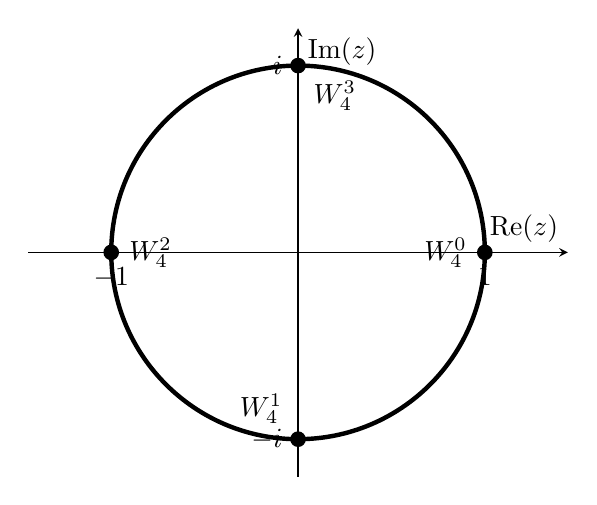
\begin{tikzpicture}
		\begin{axis}[
			xmin=-1.2,
			xmax=1.2,
			ymin=-1.2,
			ymax=1.2,
			axis equal,
			ytick={1,-1},
			xtick={1,-1},
			yticklabels={$i$,$-i$},
			axis lines=middle,
			xlabel=Re($z$),
			ylabel=Im($z$),
			disabledatascaling]
			\draw[black,ultra thick] (0,0) circle [radius=1];
			\node[circle,fill,inner sep=2pt,label=below right:$W_4^3$] at (0,1) {};
			\node[circle,fill,inner sep=2pt,label=left:$W_4^0$] at (1,0) {};
			\node[circle,fill,inner sep=2pt,label=above left:$W_4^1$] at (0,-1) {};
			\node[circle,fill,inner sep=2pt,label=right:$W_4^2$] at (-1,0) {};
		\end{axis}
	\end{tikzpicture}
\end{figure}
According to Eq.\ref{dft}, for $\forall\;k=0,1,\ldots,N-1$ we will have
$$ X_k=\sum_{n=0}^3(-i)^{kn}x_n=(-i)^{0}x_0+(-i)^{k}x_1+(-i)^{2k}x_2+(-i)^{3k}x_3$$
which is equal to 
$$ x_0+(-i)^kx_1+(-1)^kx_2+i^kx_3.$$

Our complete dicrete Fourier transform will then be:
\begin{align*}
	&X_0=x_0+x_1+x_2+x_3\\
	&X_1=x_0-ix_1-x_2+x_3\\
	&X_2=x_0-x_1-x_2-x_3\\
	&X_3=x_0+ix_1-x_2-ix_3.\\
\end{align*}

This operation is a complex multiply-add whose complexity can be better visualized if we represent it as a matrix multiplication between a matrix of twiddle factors and a column vector of input numbers.

$$
\mathbf{X}=\begin{bmatrix}X_0\\
	X_1\\
	X_2\\
	X_3\\\end{bmatrix}=\begin{bmatrix}
	W_4^{0\cdot 0} & W_4^{0\cdot 1} & W_4^{0\cdot 2} & W_4^{0 \cdot 3} \\
	W_4^{1\cdot 0} & W_4^{1\cdot 1} & W_4^{1\cdot 2} & W_4^{1 \cdot 3} \\
	W_4^{2\cdot 0} & W_4^{2\cdot 1} & W_4^{2\cdot 2} & W_4^{2 \cdot 3} \\
	W_4^{3\cdot 0} & W_4^{3\cdot 1} & W_4^{3\cdot 2} & W_4^{3 \cdot 3} \\ 
\end{bmatrix}\begin{bmatrix}
	x_0\\
	x_1\\
	x_2\\
	x_3\\
\end{bmatrix}.
$$
\end{example}

From this "direct" DFT calculation we can see how, further than the matrix multiplication, we must calculate $N\times N$ twiddle factors, which is a $\mathcal{O}(N^2)$ complexity operation. \par
We can then devise a python code that calculates the DFT of a vector with this "direct" approach.
\begin{py}
	def direct_dft(x):
	#number of numbers in input
	N = len(x)
	#array of numbers from 0 to N-1
	n = list(range(0,N)) 
	#"vertical" array of numbers from 0 to N-1 (actually a list of lists)
	k = [[item] for item in n] 
	
	#matrix of zeroes to populate with twiddle factors
	M = [[0 for col in range(N)] for row in range(N)] 
	#proceed to populate the twiddle factor matrix
	for i in range(N):
	for j in range(N):
	M[i][j]=np.exp(-2j*np.pi*i*j/N)
	
	#initialize result vector
	res = [0 for item in range(N)]
	#perform "reduced" matrix multiplication (since we know the second matrix is Nx1)
	for i in range (N):
	for j in range(N):
	res[i] += M[i][j] * x[j]
	return res
\end{py}

\subsection{A possible step further: Iterative Fast Fourier Transform Algorithm}
If we could arrange from the start the input components in a order that resembles the one reached by the deepest level of recursion (that is, when $N=1$), we could create a non-recursive approach for the FFT algorithm that works "bottom up". The idea behind this algorithm is the following:
\begin{enumerate}
\item we store in an array $A[0,\ldots,n-1]$ in the order in which they appear in the leaves of the recursion tree;
\item we take the elements in pairs, applying the butterfly operation that multiplies/adds two inputs with the twiddle factor to obtain $X_k=\text{evenFFT}_k+e^{-i\frac{2\pi}{N}k}\cdot \text{oddFFT}_k$ and $X_{k+\frac{N}{2}}=\text{evenFFT}_k-e^{-i\frac{2\pi}{N}k}\cdot \text{oddFFT}_k$. This will provide us with $N/2$ size 2 DFTs of each pair;
\item we replace the pairs in the array with their DFTs;
\item we take these $N/2$ DFTs (of size $2$ each) in pair and we compute the DFT of the $N/4$ groups of 4 input each that sit at the upper level in the recursion tree. This operation will apply two butterfly operations (since we are dealing with inputs of length 4);
\item we write these $N/4$ size 4 DFTs in the array;
\item we iterate the procedure untile the array holds 2 size $N/2$ DFTs, which we can combine using $N/2$ butterfly operations to obtain out final $N$ size DFT.
\end{enumerate}
To do this, we must firstly fill an array wtih the input component in the particular order that they appear in the leaves of the recursion graph. Let's examine the ordere in which the input components end up.\begin{center}
\begin{tabular}{|c| c c c c c c c c|}
    \hline
Original index &0 &1 &2 &3 &4 &4 &6 &7\\
\hline
Final index &0 &4 &2 &6 &1 &5 &2 &7\\
\hline
Original index (binary) &000 &001 &010 &011 &100 &101 &110 &111\\
\hline
Final index (binary) &000 &100 &010 &110 &001 &101 &011 &111\\
\hline
\end{tabular}\end{center}
We can see that the final index is the \textit{bit-reversed}\footnote{\cite{introalgo} p. 913} version of the original index: that is, to obtain the final index we must reverse the order of the bits that express the original index.
\begin{py}
def reverse(num, size):
result = 0
for _ in range(size): #shift result to the left bitwise and add the least significant bit to result
result = (result << 1) + (num & 1)
num >>= 1 #shift original number to the right bitwise (until none bits are left)
return result

def bit_reversed_order(lst):
n = len(lst)
#bit reversal depends on the size of the integer: for each index we need a number of bits equal to the number of bits used to represent the highest index
bit_size = n.bit_length() - 1 #using int class bit_length method

#note that the previous method for calculating the bit size only works because we expect the input to be a power of 2 and in binary powers of 2 are the numbers for which the number of bit needed for representation increases by 1. 
# If our input wasn't strictly in powers of 2 this method wouldn't be correct (for example, if n=5 then we would get a bit size of 2, which are too few to represent the number 4).

res = [0 for i in range(n)]
for i in range(n):
reversed_index = reverse(i, bit_size)
res[reversed_index] = lst[i]

return res
\end{py}

\end{document}

